% !TeX spellcheck = <none>
\documentclass[10pt,a4paper]{article}
\usepackage[latin1]{inputenc}
\usepackage{amsmath}
\usepackage{amsfonts}
\usepackage{amssymb}
\usepackage{graphicx}
%%% formatting the code
\usepackage{listings}



\usepackage{color}
\lstset{%
	escapeinside={(*}{*)},%
}

\newcommand{\amidstversion}{\input{../../version.txt}}

\lstset{
	frameround=fttt,
%	language=java,
	numbers=left,
	breaklines=true,
	mathescape, 
	columns=fullflexible, 
	basicstyle=\fontfamily{lmvtt}\selectfont,
	keywordstyle=\color{blue}\fontfamily{lmvtt}\selectfont, 
	numberstyle=\color{black}
}
\lstMakeShortInline[columns=fixed]|



\newcommand{\includejavasource}[1]{\lstinputlisting[language=java]{#1}}
\newcommand{\inlinejava}[1]{\lstinline[columns=fixed,language=java]{#1}}

\newcommand{\lang}[1]{}



\usepackage{hyperref}



\begin{document}

\section{Tutorial: Easy Machine Learning with Latent Variable Models in AMIDST}\label{sec:lvmodels}
%\subsection{Introduction}\label{sec:lvmodels:intro}

In AMIDST toolbox 0.4.2 the module \textit{latent-variable-models}, that contains a wide range of predefined latent variable models (see table below), was included. In this tutorial we will show how the use of this module simplifies the learning and inference processes.  In fact, you will be able to learn your model and to perform inference with a few lines of code.


\begin{figure}[h!]
	\centering
	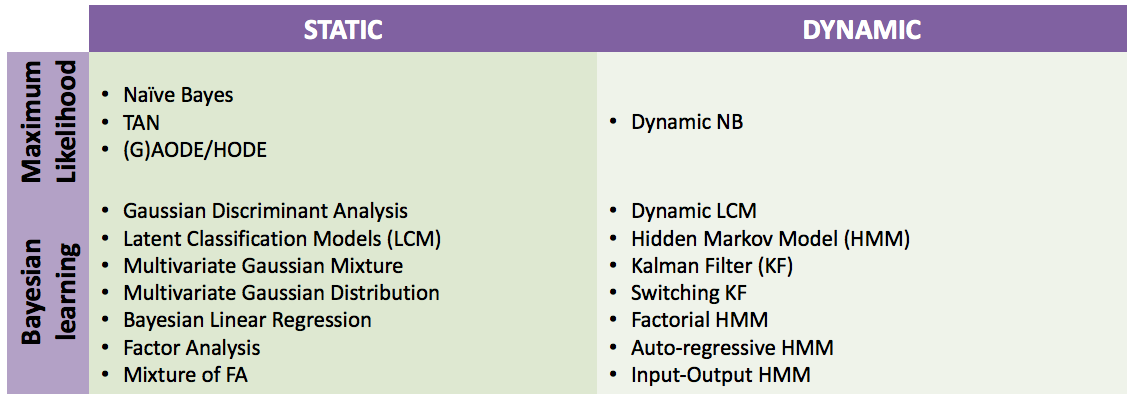
\includegraphics[width=13cm]{img/amidstModels.png}
	\caption{Set of predefined latent variable models in AMIDST}
	\label{fig:lvmodels:amidstModels}	
\end{figure}


Besides of the simplicity, the required code for learning a latent variable model is also flexible: you will be able to change the learnt model or the inference algorithm just with some slight modfications in the code. Another advantage of using AMIDST for learning one of the predefined models is that the procedure is traparent to the format of your training data: you will use the same methods regardless of learning from a local or a distributed dataset (with Flink). Note that this last feature was included in the version 0.5.0 of the toolbox.

\subsection{Setting up}

%Requirements, Project example, overview, project structure
In order to follow this tutorial, you will need to have the java 8 (i.e. SDK 1.8 or higher) installed in your system. For more details about the system requirements, see this \href{../GettingStarted/requirements.html}{link}. Additionally, you can download a ready-to-use IntelliJ maven project with all the code examples in this tutorial. For that, use the following command:

\begin{verbatim}
$ git clone https://github.com/amidst/tutorial.git      
\end{verbatim}


Alternativelly, you would rather create a new maven project or use an existing one. For that, you might check the \href{../GettingStarted/index.html}{Getting Started} page.\newline 

Note that this project does not contain any AMIDST source or binary, it only has some .java files using the AMIDST functionallity. Instead, each of the AMIDST modules are provided through maven. Doing that, the transitive dependences of the AMIDST toolbox are also downloaded in a transparent way for the user. An scheme of this idea is shown below:

 
\begin{figure}[h!]
	\centering
	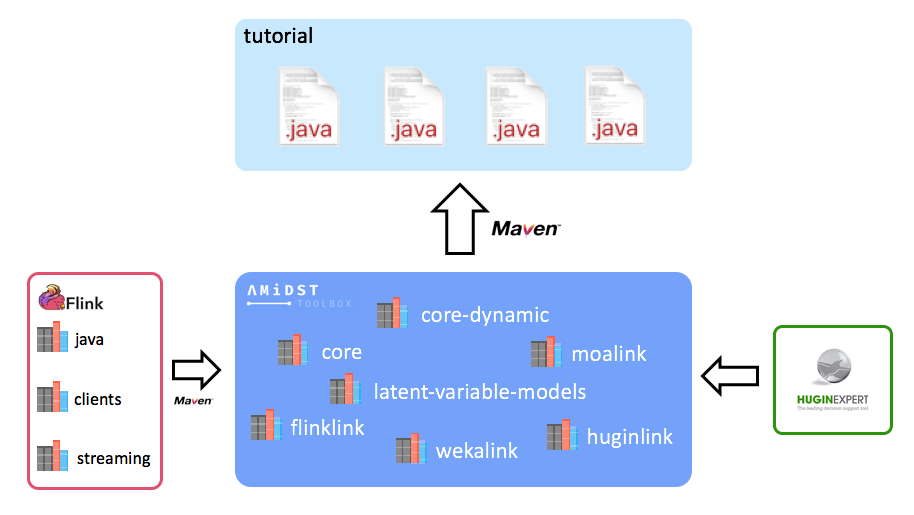
\includegraphics[width=13cm]{img/overview.png}
	\caption{Set of predefined latent variable models in AMIDST}
	\label{fig:lvmodels:overview}	
\end{figure}


\newpage 
If we open the downloaded project, we will see that it contains the following relevant folders and files:

\begin{itemize}
	\item \textbf{datasets}: folder with local and distributed datasets used in this tutorial in ARFF format.
	\item \textbf{doc}: folder containing documentation about this tutorial.
	\item \textbf{lib}: folder for storing those libraries not available through maven.
	\item \textbf{src/main/java}: folder with all the code example.
	\item \textbf{pom.xml}: this is the maven configuration file where the AMIDST dependencies are defined.
\end{itemize}


%dependencies
In the pom.xml file of the downloaded project, only the module called \textit{latent-variable-models} is linked. However some other AMIDST are also loaded as \textit{latent-variable-models} module depends on them. This is the case of the modules called \textit{core}, \textit{core-dynamic}, \textit{flinklink}, etc. You can see the full list of dependencies in the \textbf{maven project panel}, usually located on the right side of the window (see image below). If dependencies are not automatically downloaded, click on \textbf{Upload} button. It is recommended to download the sources and java 


\begin{figure}[h!]
	\centering
	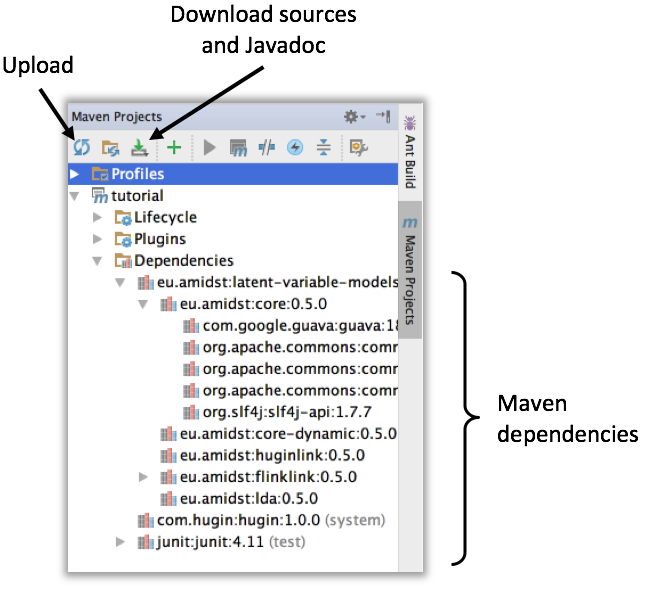
\includegraphics[width=10cm]{img/mavenpanel.png}
	\caption{Maven project panel showing the list of dependencies}
	\label{fig:lvmodels:mavenpanel}	
\end{figure}

\newpage 
\subsection{Static Models}\label{sec:lvmodels:static}
\subsubsection{Learning and saving to disk}\label{sec:lvmodels:static:learning}


Here we will see how can we learnt a static model from a local dataset (non-distributed). In particular, we will use the financial-like dataset \textbf{datasets/simulated/cajamar.arff} containing 4 continuous (normal distributed) variables. From this data,  a \textit{Factor Analysis} model will be learnt. In short, this model aims to reduce the dimensionality of a set of observed continuous variables by expressing them as combination of gaussians. A synthesis of this process is shown in the image below where: $X1, X2, X3$ and $X4$ are the observed variables and $H1, H2$ and $H3$ are the latent variables representing the combination of gaussians.

\begin{figure}[h!]
	\centering
	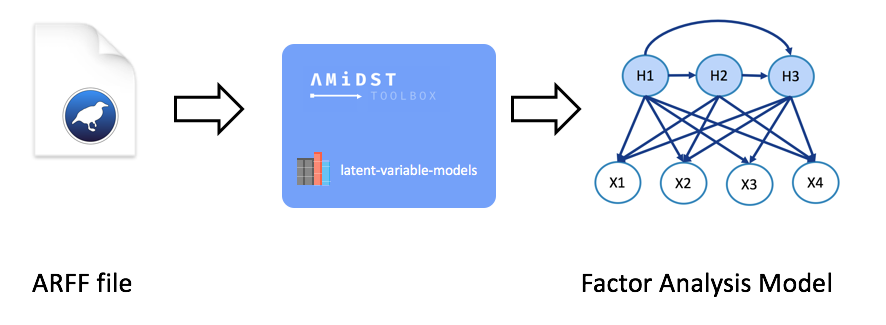
\includegraphics[width=10cm]{img/staticlearning.png}
	\caption{Static learning process}
	\label{fig:lvmodels:static:learning:scheme}	
\end{figure}


Note that the required functionality for learning the predefined model is provided by the module \textit{latent-variable-models}. A code-example for learning a factor analysis model is shown below.



\includejavasource{../../../../extensions/tutorials/src/main/java/eu/amidst/tutorial/usingAmidst/examples/StaticModelLearning.java}
\href{https://github.com/amidst/tutorial/blob/master/src/main/java/eu/amidst/tutorial/usingAmidst/examples/StaticModelLearning.java}{See on GitHub}
\vspace{3mm}


For learning any of the available static models, we create an object of any of the classes inheriting from the class \textit{Model}. These classes encapsulates all the fuctionality for learning/updating a latent-variable model. For example, in the code above we create an object of the class \textit{FactorAnalysis} which is actually stored as \textit{Model} object. The flexibility of the toolbox is due to this hierarchical desing: if we aim to change the model learnt from our data, we simply have to change the constructor used (assuming that our data also fits the constraints of the new model). For example, if we aim to learn a mixture of factor analysers instead, we simply have to replace the line 

\begin{verbatim}
Model model = new FactorAnalysis(data.getAtributes());
\end{verbatim}

\noindent by

\begin{verbatim}
Model model = new MixtureOfFactorAnalysers(data.getAtributes());
\end{verbatim}

\noindent Note that the method for learning the model, namely \textit{Model::updateMode(DataStream<DataInstance>)} will always be the same regardless of the particular type of static model.\newline 

The actual learnt model is an object of the class \textit{BayesianNetwork} which is stored as a member variable of \textit{Model}. Thus, for using the network, we simply have to extract with the method \textit{Model::getModel()}. One of the actions we can perform with it is saving it into the local file system. For saving it in \textit{.bn} format:

\begin{verbatim}
BayesianNetworkWriter::save(BayesianNetwork bn, String path)
\end{verbatim}

\noindent Alternatively, and assuming that we have the hugin library available, we can also save it in \textit{.net} format:

\begin{verbatim}
BayesianNetworkWriteToHuginr::save(BayesianNetwork bn, String path)
\end{verbatim}



\subsubsection{Learning from Flink}\label{sec:lvmodels:static:flinklearning}

In previous section we showed how the AMIDST toolbox can be used for learning a static model from a non-distributed dataset. In addition, you can use the pre-defined models to process massive data sets in a distributed computer cluster using \textbf{Apache Flink}. In particular, the model can be learnt from a \textit{distributed ARFF folder} or from a file  accesible via a HDFS url. A scheme of the learning process is shown below.




%%Poner imagen
\begin{figure}[h!]
	\centering
	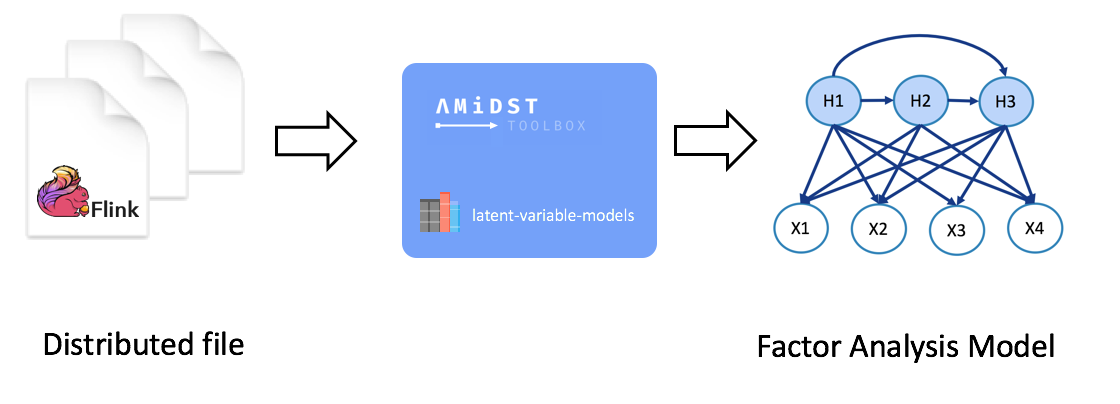
\includegraphics[width=10cm]{img/distributedlearning.png}
	\caption{Distributed learning process scheme}
	\label{fig:lvmodels:static:flinklearning:scheme}	
\end{figure}

A code example for learning from Flink is shown below. Note that it only differs from the one in previous section in lines 25 to 33. In these lines, the Flink session is configurated and the stream is loaded, which is managed with an object of the class \textit{DataFlink} (instead of \textit{DataStream}). 

\includejavasource{../../../../extensions/tutorials/src/main/java/eu/amidst/tutorial/usingAmidst/examples/StaticModelFlink.java}
\href{https://github.com/amidst/tutorial/blob/master/src/main/java/eu/amidst/tutorial/usingAmidst/examples/StaticModelFlink.java}{See on GitHub}
\vspace{3mm}


In previous example, the distributed dataset is stored in our local file system. Instead, we might need to load from a distributed file system. For that, simply replace the string indicating the path. That is, replace


\begin{verbatim}
String filename = "datasets/simulated/cajamarDistributed.arff"
\end{verbatim}


\noindent by


\begin{verbatim}
String filename = "hdfs://distributed-server/path-to-file"
\end{verbatim}



\subsubsection{Inference}\label{sec:lvmodels:static:inference}



Making probabilistic inference in BNs (a.k.a \textit{belief updating}) consists of the computation of the posterior probability distribution for a set of variables of interest given some evidence over some other variables (see image below). 


%%Poner imagen
\begin{figure}[h!]
	\centering
	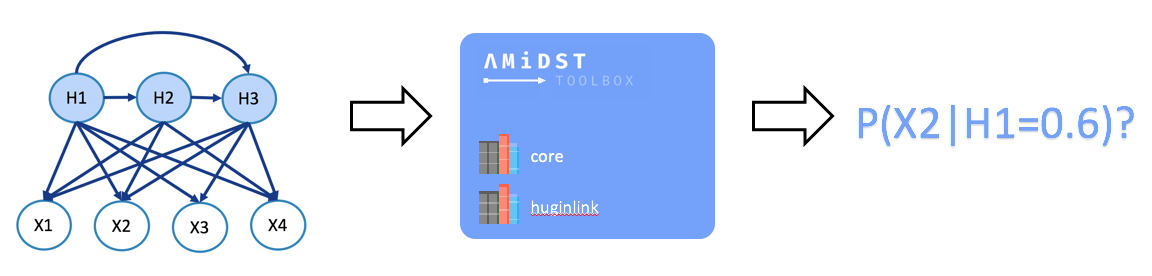
\includegraphics[width=10cm]{img/staticinference.png}
	\caption{Learning process scheme}
	\label{fig:lvmodels:static:inference:scheme}	
\end{figure}

The inference process is the same regardless of the way we have learnt our model: we simply have to obtain the BN learnt (stored as an object of the class \textit{BayesianNetwork}), set the target variables and the evidence. As an example, let us consider the following code:



\includejavasource{../../../../extensions/tutorials/src/main/java/eu/amidst/tutorial/usingAmidst/examples/StaticModelInference.java}
\href{https://github.com/amidst/tutorial/blob/master/src/main/java/eu/amidst/tutorial/usingAmidst/examples/StaticModelInference.java}{See on GitHub}

Note that the learning algorithm can be easily changed by simply modifying line 35 where \textit{VMP algorithm}. If we aim to use \textit{Importance Sampling algorithm}, replace such line with:

\begin{verbatim}
	InferenceAlgorithm infer = new ImportanceSampling();
\end{verbatim}  

Alternatively, we can use \textit{Hugin Inference algorithm} (assuming that we have the corresponding libraries):

\begin{verbatim}
InferenceAlgorithm infer = new HuginInference();
\end{verbatim}  



\subsubsection{Custom static model}\label{sec:lvmodels:static:custom}

It could happend that your model of interest is not predifined. In that case you can implement it yourself. For that purpose, create a new class inheriting the class \textit{Model}. Then, add the code to the constructor with an object \textit{Attributes} as input parameter, and the code of the method \textit{void buildDAG()}. This last method is called before learning process and creates the object representing the DAG. As an example, the code below shows how to create a custom Gaussian Mixture.


\includejavasource{../../../../extensions/tutorials/src/main/java/eu/amidst/tutorial/usingAmidst/practice/CustomGaussianMixture.java}
\href{https://github.com/amidst/tutorial/blob/master/src/main/java/eu/amidst/tutorial/usingAmidst/practice/CustomGaussianMixture.java}{See on GitHub}


\subsection{Dynamic Models}\label{sec:lvmodels:dynamic}
\subsubsection{ Learning and saving to disk }\label{sec:lvmodels:dynamic:learning}

When dealing with temporal data, it might be advisable to learn a dynamic model. The module \textit{latent-variable-models} in AMDIST also suports such kinds of models. For that the classes inheriting \textit{DynamicModel} will be used. A synthesis of the learning process is shown below.\newline 



\begin{figure}[h!]
	\centering
	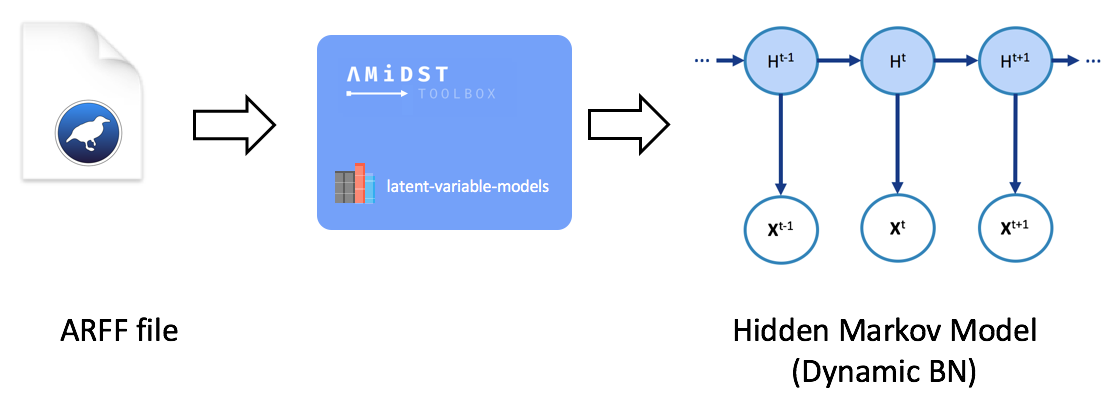
\includegraphics[width=10cm]{img/dynamicLearning.png}
	\caption{Learning process scheme of a dynamic model}
	\label{fig:lvmodels:dynamic:learning:scheme}	
\end{figure}


A code-example is given below. Here, a \textit{Hidden Markov Model (HMM)} is learnt from a financial dataset with temporal information. Note the difference within the static learning is the way the dataset is loaded: now, it is handled with an object of the class \textit{DataStream<DynamicDataInstance>}. Finally, the DBN learnt is saved to disk with the method \textit{DynamicBayesianNetworkWriter::save(String pathFile)}.\newline 


\includejavasource{../../../../extensions/tutorials/src/main/java/eu/amidst/tutorial/usingAmidst/examples/DynamicModelLearning.java}
\href{https://github.com/amidst/tutorial/blob/master/src/main/java/eu/amidst/tutorial/usingAmidst/examples/DynamicModelLearning.java}{See on GitHub}

\subsubsection{Inference}

In the following code-example, the inference process of dynamic models is illustrated. First, a DBN is loaded from disk (line 24). Then, a dynamic dataset is loaded for testing our model (lines 29 to 30). Then the inference algorithm and target variables are set. In the final loop, the inference is perform for each data instance.\newline 

\includejavasource{../../../../extensions/tutorials/src/main/java/eu/amidst/tutorial/usingAmidst/examples/DynamicModelInference.java}
\href{https://github.com/amidst/tutorial/blob/master/src/main/java/eu/amidst/tutorial/usingAmidst/examples/DynamicModelInference.java}{See on GitHub}


Note that the inference algorithm can be easily change if line 33 is modified by replacing it with:

\begin{verbatim}
InferenceAlgorithmForDBN = new FactoredFrontierForDBN(new VMP());
\end{verbatim}


\subsubsection{Custom dynamic model}\label{sec:lvmodels:dynamic:custom}

Like for static models, we might be interested in creating our own dynamic models. In this case, you will have to create a class inheriting \textit{DynamicModel}. Here below an example of a custom \textit{Kalman Filter} is given.

\includejavasource{../../../../extensions/tutorials/src/main/java/eu/amidst/tutorial/usingAmidst/practice/CustomKalmanFilter.java}
\href{https://github.com/amidst/tutorial/blob/master/src/main/java/eu/amidst/tutorial/usingAmidst/practice/CustomKalmanFilter.java}{See on GitHub}




\end{document}